\documentclass[fleqn]{article}
\usepackage[english]{babel}
\usepackage{amsmath}
\usepackage{amsthm}
\usepackage{graphicx}
\usepackage[utf8]{inputenc}

%%%%%%%% MARGIN
\usepackage[left=1in, right=1in, top=0.8in, bottom=0.8in]{geometry}

%%%%%%%% NO PARAGRAPH INDENT
% https://tex.stackexchange.com/questions/27802/set-noindent-for-entire-file
\setlength\parindent{0pt}

%%%%%%%% SUB-FIGURE PACKAGE
\usepackage{subcaption}

%%%%%%%% HYPERREF PACKAGE
\usepackage{hyperref}
\hypersetup{linkcolor=blue}
\hypersetup{citecolor=blue}
\hypersetup{urlcolor=blue}
\hypersetup{colorlinks=true}

%%%%%%%% MULTI-COLUMNS PACKAGE
\usepackage{multicol}

%%%%%%%% SETS DEFINITIONS
\usepackage{amssymb}
%%%% Important sets
\renewcommand{\O}{\mathbb{O}}
\newcommand{\N}{\mathbb{N}}
\newcommand{\Z}{{\mathbb{Z}}}
\newcommand{\Q}{{\mathbb{Q}}}
\newcommand{\R}{{\mathbb{R}}}

%%%% Statistics
\newcommand{\E}[1]{\mathbb{E}\left[#1 \right]}
\newcommand{\V}[1]{\mathrm{Var}\left[#1 \right]}

%%%% Lambda Calculus Symbols
\newcommand{\dneq}{\,\, \# \,\,}
\renewcommand{\S}{\pmb{\mathrm{S}}}
\newcommand{\I}{\pmb{\mathrm{I}}}
\newcommand{\K}{\pmb{\mathrm{K}}}
\newcommand{\ch}[1]{\ulcorner #1 \urcorner}

%%%% Ordinal Lambda Calculus Symbols
\newcommand{\ordAlph}{\Sigma_{\text{Ord}}}
\newcommand{\termOrd}{\text{Term}_\text{Ord}}
\newcommand{\fl}{\mathrm{fl}}
\newcommand{\sk}{\mathrm{sk}}

%%%% Superscript to the left
% https://latex.org/forum/viewtopic.php?t=455
\usepackage{tensor}
\newcommand{\app}[3]{\tensor*[^{#1}]{\left(#2, #3\right)}{}}

%%%% Make optional parameter
% https://tex.stackexchange.com/questions/217757/special-behavior-if-optional-argument-is-not-passed
\usepackage{xparse}
\NewDocumentCommand{\cx}{o}{
  \IfNoValueTF{#1}
  {\left[\quad\right]}
  {\left[\, #1 \,\right]}
}

%%%%%%%% LOGIC TREES
\usepackage{prftree}

%%%%%%%% SPLIT EQUATIONS
% https://tex.stackexchange.com/questions/51682/is-it-possible-to-pagebreak-aligned-equations
\allowdisplaybreaks

%%%%%%%% CODE RENDERING
% Compile with flag -shell-escape
% \usepackage{minted}

%%%%%%%% EXAM PACKAGE
\usepackage{mathexam}

%%%%%%%% CHANGE MARGINS ITEMIZE
\usepackage{enumitem}

\usepackage{float}

%%%%%%%% START DOCUMENT

\ExamClass{NON PARAMETRIC STATISTICS}
\ExamName{FINAL EXAM}
\ExamHead{\today}

\let\ds\displaystyle

\begin{document}
 \vspace{0.3cm}
   % Information of the student
   \begin{itemize}[leftmargin=6.25cm, labelsep=0.5cm]

     \item[\textit{Name}] \scalebox{1.2}{Juan Sebastián Cárdenas Rodríguez} % Name
     \item[\textit{Code}] 201710008101 % Code

   \end{itemize}
\vspace{0.3cm}

% Each of the items to solve
\begin{enumerate}[label=\alph*)]
  \item Each Empirical Continuous Distribution Function (ECDF) is shown in
    Figure \ref{fig:ecdfs}.
  \begin{figure}[H]
    \centering
    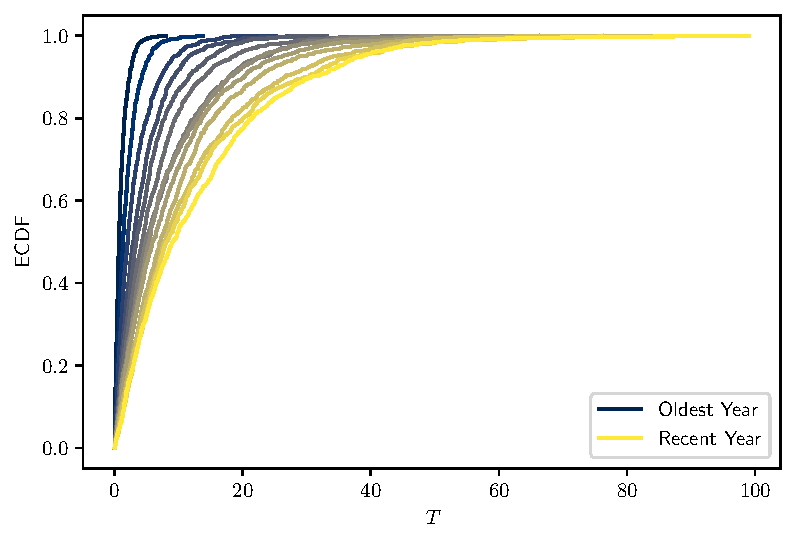
\includegraphics[scale=.5]{../figs/ecdfs.pdf}
    \caption{ECDF for each year.}
    \label{fig:ecdfs}
  \end{figure}
    It is easily seen that there is an improvement of the life span of the
    devices through time. This can be justified as recent years have a ECDF
    lower than the ones from oldest years. This is a desired behavior because,
    if it happens that for a time $t$ it occurs that
    \[
      \hat{F}_{n}(t) \le \hat{F}_{1}(t)
    \]
    Then, it occurs that the device has less probability that its lifespan is
    less than time $t$ (i.e. has more probability of having a bigger lifespan).
    In these manner, the intervals where the first year ECDF is bigger than the
    last year it means that a device has more probability of having a smaller
    lifespan.

  \item The confidence bands of the ECDF of the first year, with a confidence of
  90\% ($\alpha=0.1$) are shown in Figure \ref{fig:bands}.
  \begin{figure}[H]
    \centering
    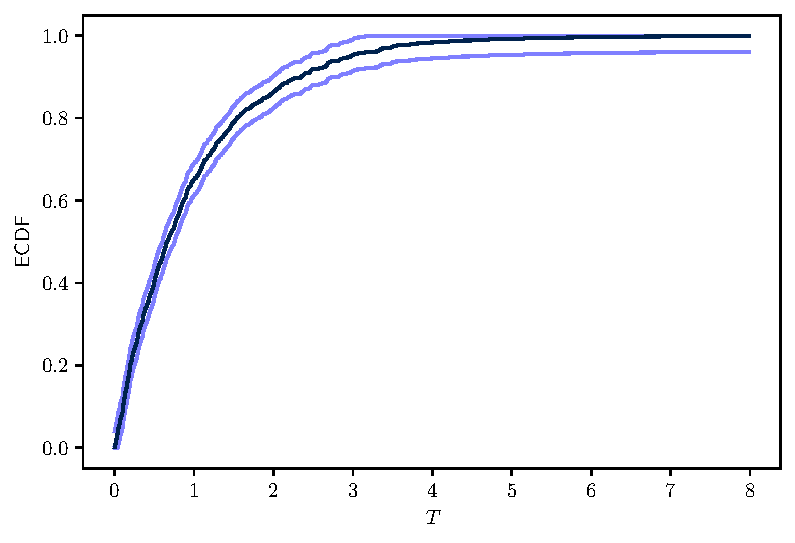
\includegraphics[scale=.5]{../figs/ecdf_bands}
    \caption{Confidence bands for ECDF of first year.}
    \label{fig:bands}
  \end{figure}

  \item The comparisons of the ECDF and the estimated density can be found
    Figure \ref{fig:comp}. For the Kernel estimation, the bandwidth was selected
    as $h = 4$.
    \begin{figure}[H]
      \centering
      \begin{subfigure}[b]{0.4\textwidth}
        \centering
        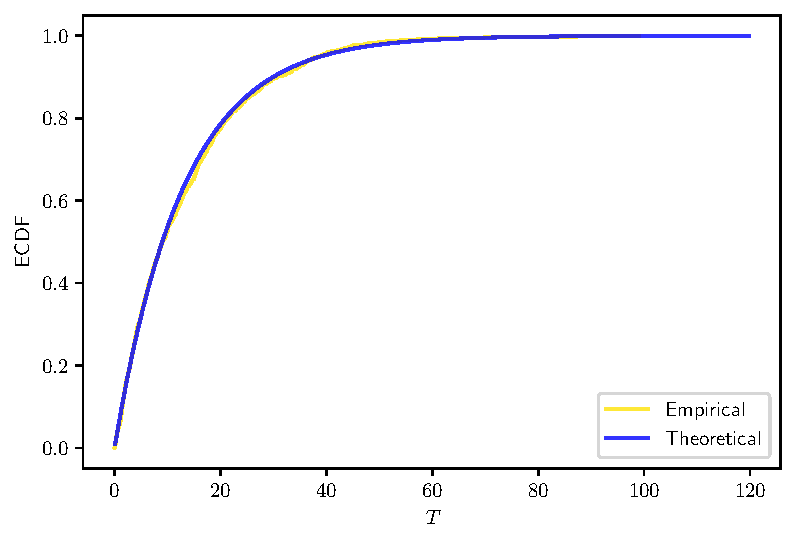
\includegraphics[scale=.5]{../figs/ecdf-vs-theo}
        \caption{ECDF comparison.}
      \end{subfigure}
      \begin{subfigure}[b]{0.4\textwidth}
        \centering 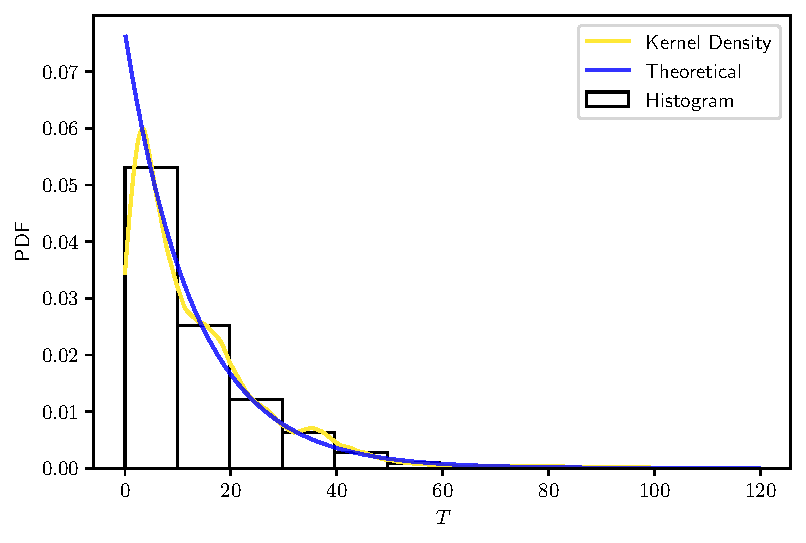
\includegraphics[scale=0.5]{../figs/pdf-vs-theo}
        \caption{EPDF comparison.}
      \end{subfigure}
      \caption{Comparisons to the proposed distribution}
      \label{fig:comp}
    \end{figure}
    It is considered that there is a good fit of both distributions, as the ECDF
    is very close to the proposed distribution. Furthermore, as the size of the
    sample is considerably big, it would already converge to its theoretical
    distribution. Hence, if the exponential distribution was not the real
    distribution of the data the ECDF would be a lot different.

    To show computationally the Glivenko Cantelli theorem, the data was
    sampled for different percentages. To do that, 1000 samples where generated
    by randomly extracting a percentage $p$ of the original data such that
    $0.01 \le p \le 1$. Then, the ECDF was calculated for that sample and the
    difference is calculated. The result of this experiment can be seen in
    Figure \ref{fig:gcv}.
    \begin{figure}[H]
      \centering
      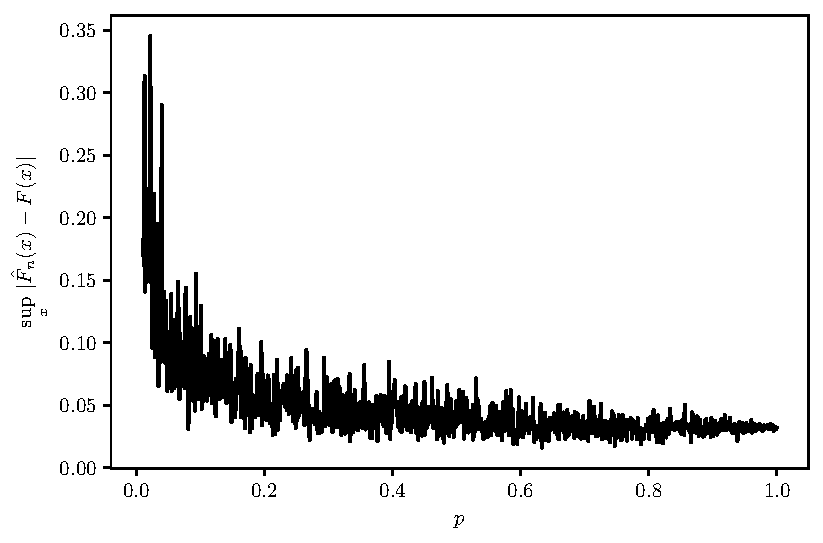
\includegraphics[scale=.5]{../figs/glivenko-cantelli}
      \caption{Glivenko Cantelli theorem visualization.}
      \label{fig:gcv}
    \end{figure}

    It is clear that when the $n$ tends to be bigger, then the difference
    between the ECDF and the theoretical distribution becomes smaller. Hence,
    the Glivenko Cantelli theorem is satisfied for the data and the selected
    distribution.

  \item It is known that if the $\mathrm{MSE}$ converges to 0 when
    $n \rightarrow \infty$ then succession of random variables converges in
    probability. Let's calculate the limit:
    \begin{align*}
      \lim_{n \rightarrow \infty} \mathrm{MSE}(X_{n}, b)
      &= \lim_{n \rightarrow \infty} \left(\mathrm{Bias}^{2}(X_{n}, b) + \V{X_n} \right)\\
      &= \lim_{n \rightarrow \infty} \left(\E{X_{n}} - b\right)^{2} +
        \lim_{n \rightarrow \infty} \V{X_{n}} \\
      &= \left(b - b\right)^{2} \\
      &= 0
    \end{align*}
    Hence, it can be concluded that $X_{n} \xrightarrow[]{\,\, P \,\,} b$.

  \item The Bootstrap Normal Method gives an interval, with a confidence of
  95\%, for the maximum value of:
    \[
    X_{[n]} \in (6.9132, 9.05134)
    \]
    And for the variance and bias given by the Jackknife method is:
    \[
    \mathrm{Bias}_{jack} = -0.6563 \quad v_{\mathrm{jack}} = 4.338 \times 10^{-7}
    \]

  \item To make a regression for the costs of the repair of each device in the
    first year, to the respective life span of each device the Nadaraya Watson
    Kernel Regression will be used. This is done as a linear regression could
    not fully represent a regression between these two variables. In Figure
    \ref{fig:nwr}, the data and the regression estimation model can be found.
    \begin{figure}[H]
      \centering
      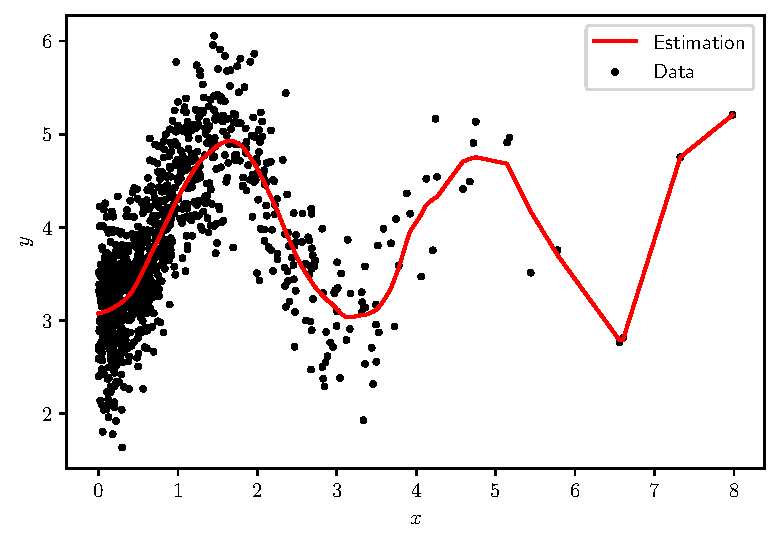
\includegraphics[scale=.5]{../figs/scatter-vs-model}
      \caption{Data and Nadaraya-Watson regression.}
      \label{fig:nwr}
    \end{figure}

    It is clear from the graph that both variables have a sine-like dependency,
    hence a linear regression could not represent fully this relationship.

  \item In Table \ref{tab:homo} the result of each homogeneity test can be seen.
    If an element in the table is 1, it means that the pair of data did not come
    from the same distribution.
    \begin{table}[H]
      \centering
      \begin{tabular}{cccccccccccccc}
        & \textbf{0} & \textbf{1} & \textbf{2} & \textbf{3} & \textbf{4} & \textbf{5} & \textbf{6} & \textbf{7} & \textbf{8} & \textbf{9} & \textbf{10} & \textbf{11} & \textbf{12} \\ \cline{2-14}
        \multicolumn{1}{l|}{\textbf{0}}  & 0          & 1          & 1          & 1          & 1          & 1          & 1          & 1          & 1          & 1          & 1           & 1           & 1           \\
        \multicolumn{1}{l|}{\textbf{1}}  & 1          & 0          & 1          & 1          & 1          & 1          & 1          & 1          & 1          & 1          & 1           & 1           & 1           \\
        \multicolumn{1}{l|}{\textbf{2}}  & 1          & 1          & 0          & 1          & 1          & 1          & 1          & 1          & 1          & 1          & 1           & 1           & 1           \\
        \multicolumn{1}{l|}{\textbf{3}}  & 1          & 1          & 1          & 0          & 1          & 1          & 1          & 1          & 1          & 1          & 1           & 1           & 1           \\
        \multicolumn{1}{l|}{\textbf{4}}  & 1          & 1          & 1          & 1          & 0          & 1          & 1          & 1          & 1          & 1          & 1           & 1           & 1           \\
        \multicolumn{1}{l|}{\textbf{5}}  & 1          & 1          & 1          & 1          & 1          & 0          & 1          & 1          & 1          & 1          & 1           & 1           & 1           \\
        \multicolumn{1}{l|}{\textbf{6}}  & 1          & 1          & 1          & 1          & 1          & 1          & 0          & 0          & 1          & 1          & 1           & 1           & 1           \\
        \multicolumn{1}{l|}{\textbf{7}}  & 1          & 1          & 1          & 1          & 1          & 1          & 0          & 0          & 1          & 1          & 1           & 1           & 1           \\
        \multicolumn{1}{l|}{\textbf{8}}  & 1          & 1          & 1          & 1          & 1          & 1          & 1          & 1          & 0          & 1          & 1           & 1           & 1           \\
        \multicolumn{1}{l|}{\textbf{9}}  & 1          & 1          & 1          & 1          & 1          & 1          & 1          & 1          & 1          & 0          & 1           & 1           & 1           \\
        \multicolumn{1}{l|}{\textbf{10}} & 1          & 1          & 1          & 1          & 1          & 1          & 1          & 1          & 1          & 1          & 0           & 0           & 1           \\
        \multicolumn{1}{l|}{\textbf{11}} & 1          & 1          & 1          & 1          & 1          & 1          & 1          & 1          & 1          & 1          & 0           & 0           & 0           \\
        \multicolumn{1}{l|}{\textbf{12}} & 1          & 1          & 1          & 1          & 1          & 1          & 1          & 1          & 1          & 1          & 1           & 0           & 0
      \end{tabular}
      \caption{Result for each homogeneity tests.}
      \label{tab:homo}
    \end{table}

    It is clear that most of the years did not pass the homogeneity test,
    highlighting the fact that the lifespan actually increased significantly as
    mention in the first question.

  \item To do a multivariate homogeneity test, a D-D plot was constructed and
    then a linear regression was constructed to find if it was close enough to
    the line $y = x$. In these manner, for the first pair of data the D-D plot
    found and the regression model can be seen in Figure \ref{fig:ddplot400}.
    \begin{figure}[ht]
      \centering
      \begin{subfigure}[b]{0.4\textwidth}
        \centering 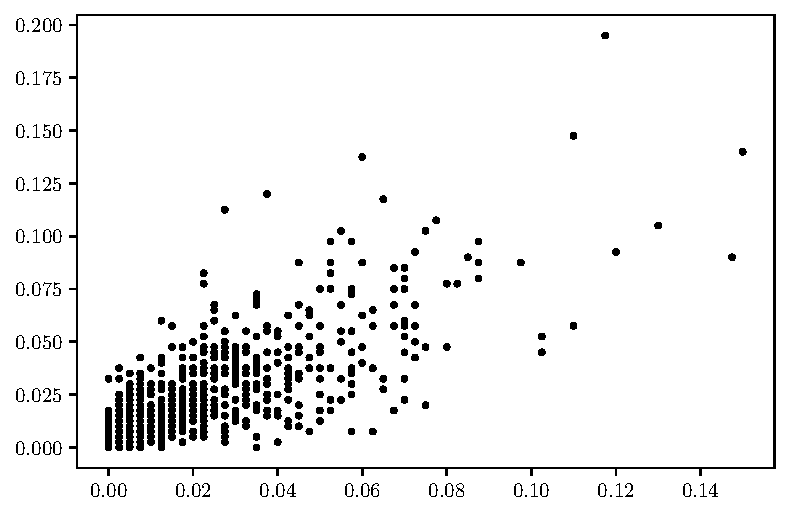
\includegraphics[scale=.5]{../figs/ddplot-400}
      \end{subfigure}
      \begin{subfigure}[b]{0.4\textwidth}
        \centering
        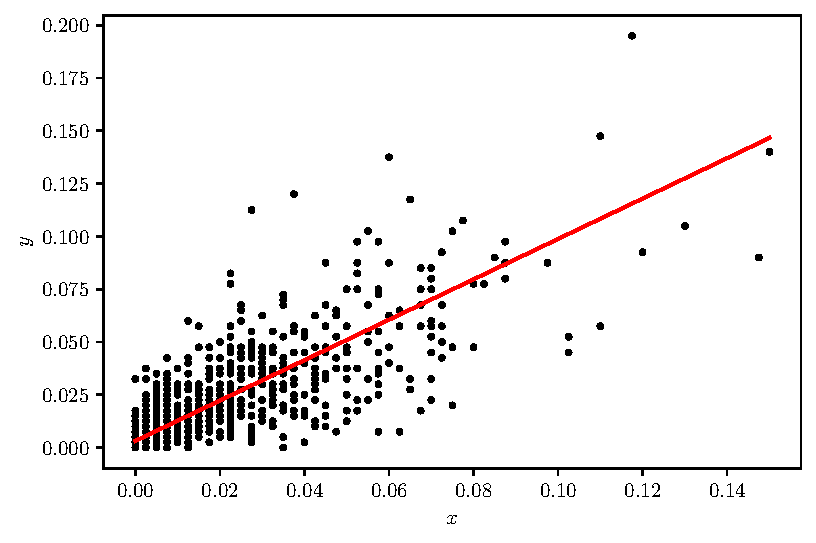
\includegraphics[scale=.5]{../figs/scatter-vs-model-ddplot-400}
      \end{subfigure}
      \caption{D-D plot for the first and last 400 devices for the first year.}
      \label{fig:ddplot400}
    \end{figure}

    Furthermore, the model obtained was:
    \[
    y = 0.9565 x + 0.0031
    \]

    It is clearly seen that this model is close enough to the proposed line. In
    these manner, it is concluded that this samples are homogeneous. On the
    other hand, the D-D plot for the first and last 5 years is shown in Figure
    \ref{fig:ddplot5}.
    \begin{figure}[H]
      \centering
      \begin{subfigure}[b]{0.45\textwidth}
        \centering
        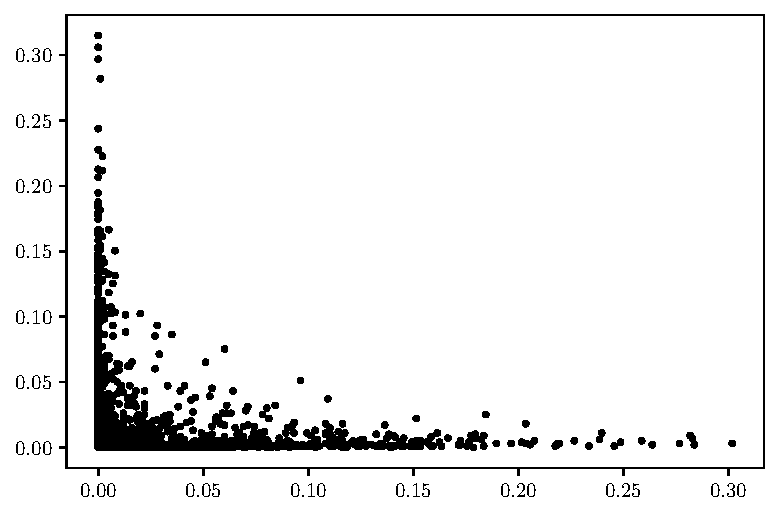
\includegraphics[scale=.5]{../figs/ddplot-5}
      \end{subfigure}
      \begin{subfigure}[b]{0.45\textwidth}
        \centering
        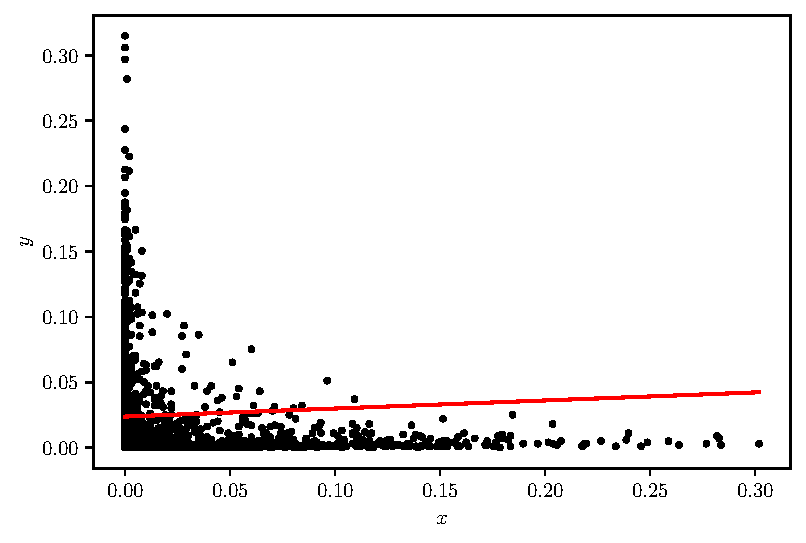
\includegraphics[scale=.5]{../figs/scatter-vs-model-ddplot-5}
      \end{subfigure}
      \caption{D-D plot for the first and last 5 years.}
      \label{fig:ddplot5}
    \end{figure}

    It is easily seen that a linear regression model can not be fitted to the
    data, as they do not have a linear dependency. In this manner, the obtained
    model for this graph is:
    \[
      y = 0.0616x + 0.0212
    \]

    Hence, it can be concluded that the first and last 5 years are not
    homogeneous. This is supported by the conclusion made in the first question.

  \item The linear regression model was constructed using six different methods,
    five of them which use robust Covariance estimation matrix. In this manner,
    to measure performance of each method three things are displayed.
    $\beta_{0}$ which should be close to 0 by the construction of the original
    model and, these two other calculations:
    \[
      D_{\beta_{1}} = \lVert \hat{\beta}_{1} - \beta_{1} \rVert_{2} \quad
      D_{y} = \lVert \hat{y} - y \rVert_{\infty}
    \]
    with $\lVert \cdot \rVert_{p}$ being the $p$-norm of a vector. With these
    calculations, its is possible to see the closeness of the estimation of the
    parameters and, furthermore, the closeness to the estimation of the whole
    output $y$. The results for each method can be seen in Table \ref{tab:lrp}.
    \begin{table}[H]
      \centering
      \begin{tabular}{llll}
        \hline
        & $D_{\beta_1}$ & $D_y$  & $\beta_0$ \\
        Least Squares & 1.44          & 185.37 & -0.43     \\
        Comedian      & 4.59          & 215.96 & 51.71     \\
        Spearman      & 3.61          & 196.09 & 51.36     \\
        Kendall       & 11.14         & 236.36 & 185.76    \\
        Fast MCD      & 21.12         & 376.29 & 340.70    \\
        Shrinkages    & 9.79          & 175.61 & 21.96     \\ \hline
      \end{tabular}
      \caption{Performance of each linear regression.}
      \label{tab:lrp}
    \end{table}

    It is seen that the closest estimation to the original parameter was done
    with the least-square linear regression model. On the other hand, the
    closest approximation to the real output was done by the Shrinkages method.
    Hence, both the Least Squares and the Shrinkages methods where the best
    estimating the original output.
\end{enumerate}
\end{document}
